\documentclass[papersize=a4,DIV=calc,twocolumn=on]{scrartcl}
\usepackage[portuguese]{babel}
\usepackage[utf8]{inputenc}
\usepackage[colorlinks,allcolors=blue]{hyperref}
\usepackage{microtype}
\usepackage{amsmath,amsfonts,amsthm}
\usepackage{graphicx}

\newcommand{\dpar}[1]{\left(#1\right)}
\newcommand{\dsqr}[1]{\left[#1\right]}

\theoremstyle{definition}
\newtheorem{ex}{Exercício}[section]

\DeclareMathOperator{\sen}{sen}

\title{Notas de Física Geral 2}

\author{Max Jáuregui}

\begin{document}
\maketitle
\tableofcontents

\section{Equilíbrio de um corpo rígido}

Considere uma partícula de massa $m$ na posição $\vec r$ sobre a qual
atua uma força $\vec F$. O \textbf{torque} da força $\vec F$ é
definido por $\vec\tau=\vec r\times\vec F$, onde $\times$ denota o
\textbf{produto vetorial} de dois vetores, o qual é definido por
\begin{equation*}
  \begin{split}
    \vec A\times\vec B&= \left|
      \begin{array}{ccc}
        \hat i&\hat j&\hat k\\
        A_x&A_y&A_z\\
        B_x&B_y&B_z
      \end{array}
    \right|\\
    &=(A_yB_z-A_zB_y)\hat i+(A_zB_x-A_xB_z)\hat j\\
    &\quad+(A_xB_y-A_yB_x)\hat k\,.
  \end{split}
\end{equation*}

A unidade do torque no sistema internacional (SI) é
$\mathrm{N}\cdot\mathrm{m}$.

\begin{ex}
  Verifique que, para uma partícula de $10\,\mathrm{kg}$ na posição
  $\vec r=\cos 30^\circ\hat i+\sen 30^\circ\hat j$ (em metros), o
  torque do peso é igual a $-49\sqrt{3}\hat k$ (em
  $\mathrm{N}\cdot \mathrm{m}$).
\end{ex}

Usaremos a notação $\dot{\vec a}$ para representar a derivada de
$\vec a$ em relação ao tempo, ou seja,
$\dot{\vec a}=\frac{d\vec a}{dt}$.

\begin{ex}
  Considere uma partícula de massa $m$ na posição $\vec r$ sobre a
  qual atua uma força $\vec F$. Definindo o \textbf{momento angular}
  de uma partícula por $\vec L=\vec r\times\vec p$, onde $\vec p$ é o
  momento linear da partícula, mostre que $\vec\tau=\dot{\vec
    L}$. Isso quer dizer que o torque da força $\vec F$ é igual à taxa
  de variação do momento angular da partícula (note a semelhança com a
  segunda lei de Newton). A unidade de momento angular no SI é
  $\mathrm{kg}\cdot\mathrm{m^2/s}$.

  \noindent\textit{Dica:} Na expressão do torque substitua $\vec F$ por
  $\dot{\vec p}$, em virtude da segunda lei de Newton
  ($\vec F=\dot{\vec p}$). Logo, utilize a identidade
  $\frac{d}{dt}(\vec r\times\vec p)=\dot{\vec r}\times\vec p+\vec
  r\times\dot{\vec p}$ e use o fato de que
  $\dot{\vec r}\times\vec p=0$, pois o vetor velocidade $\dot{\vec r}$
  é paralelo a $\vec p$.
\end{ex}

\begin{ex}
  Considere duas partículas de massas $m_1$ e $m_2$ sobre as quais
  atuam forças externas $\vec F_1$ e $\vec F_2$ respectivamente. Além
  das forças externas, há forças internas $\vec F_{12}$ (sobre a
  partícula $1$) e $\vec F_{21}$ (sobre a partícula $2$) devido a
  interação das partículas (por exemplo, interação gravitacional ou
  elétrica), as quais são paralelas ao vetor $\vec r_1-\vec
  r_2$. Mostre que
  \begin{equation}
    \label{eq:1}
    \begin{split}
      \vec F_1+\vec F_2&=\dot{\vec p}_1+\dot{\vec p}_2\\
      \vec\tau_1+\vec\tau_2&=\dot{\vec L}_1+\dot{\vec L}_2\,.
    \end{split}
  \end{equation}

  \noindent\textit{Dica:} Segue da segunda lei de Newton que
  \begin{equation}
    \label{eq:2}
    \begin{split}
      \vec F_1+\vec F_{12}&=\dot{\vec p}_1\\
      \vec F_2+\vec F_{21}&=\dot{\vec p}_2\,.
    \end{split}
  \end{equation}
  Somando essas equações e usando a terceira lei de Newton
  ($\vec F_{12}=-\vec F_{21}$), obtém-se a primeira equação
  em~(\ref{eq:1}). Para se obter a segunda equação em~(\ref{eq:1}),
  multiplicam-se vetorialmente à esquerda as equações~(\ref{eq:2})
  pelos vetores posição $\vec r_1$ e $\vec r_2$ respectivamente. Logo,
  somam-se as equações obtidas e usa-se o fato de que
  $(\vec r_1-\vec r_2)\times\vec F_{12}=\vec 0$.
\end{ex}

O exemplo anterior pode ser generalizado sem realizar nenhuma
alteração fundamental para o caso de um sistema de $n$
partículas. Nesse caso vamos ter que
\begin{equation}
  \label{eq:3}
  \begin{split}
    \vec F_{\mathrm{ext}}&=\dot{\vec p}\\
    \vec \tau_{\mathrm{ext}}&=\dot{\vec L}\,,
  \end{split}
\end{equation}
onde $\vec F_{\mathrm{ext}}=\vec F_1+\cdots+\vec F_n$ é a força
externa total sobre o sistema, $\vec p=\vec p_1+\cdots+\vec p_n$ é o
momento linear total do sistema,
$\vec\tau_{\mathrm{ext}}=\vec\tau_1+\cdots+\vec\tau_n$ é o torque
externo total sobre o sistema e $\vec L=\vec L_1+\cdots+\vec L_n$ é o
momento angular total do sistema.

Um \textbf{corpo rígido} é um corpo não pontual que não se deforma. O
fato de um corpo rígido não se deformar equivale a dizer que a
distância entre dois pontos quaisquer do corpo é uma constante.

Para estudar a dinâmica de um corpo rígido, podemos dividir ele em $n$
partes pequenas e assim considerar o corpo rígido como um sistema de
$n$ corpos. Se a massa da $i$-ésima parte é $\Delta m_i$, sua posição
é $\vec r_i$ e sua velocidade é $\vec v_i$, o momentum total do
sistema é
$$\vec p=\sum_{i=1}^n\vec v_i\Delta m_i$$
e o momento angular total do sistema é
$$\vec L=\sum_{i=1}^n(\vec r_i\times\vec v_i)\Delta m_i\,.$$
Considerando que o número de partes $n$ tende ao infinito e
simultaneamente a massa de cada parte tende a zero, as somas
anteriores tornam-se integrais. Dessa maneira, encontramos que o
\textbf{momento linear do corpo rígido} é dado por
\begin{equation}
  \label{eq:4}
  \vec p=\int \vec v\,dm
\end{equation}
e o \textbf{momento angular do corpo rígido} por
\begin{equation}
  \label{eq:5}
  \vec L=\int (\vec r\times\vec v)\,dm\,,
\end{equation}
onde as integrais são sobre toda a massa do corpo rígido.

As Eqs.~(\ref{eq:3}) continuam valendo da mesma forma para um corpo
rígido, levando em conta que $\vec p$ e $\vec L$ são dadas pelas
Eqs.~(\ref{eq:4}) e~(\ref{eq:5}).

O movimento de um corpo rígido pode ser estudado analisando
separadamente os movimentos de translação e de rotação em torno de um
eixo que passa pelo corpo.

\begin{ex}
  Considere um corpo rígido de massa $M$ que realiza um movimento de
  translação pura com velocidade $\vec v$. Mostre que nesse caso
  \begin{equation}
    \label{eq:6}
    \vec p=M\vec v\quad\text{e}\quad \vec L=\vec R\times\vec p\,,
  \end{equation}
  onde
  $$\vec R=\frac{1}{M}\int \vec r\,dm$$
  é a posição do \textbf{centro de massa} do corpo.

  \noindent\textit{Dica:} Quando um corpo rígido realiza um movimento de translação pura, todos os pontos do corpo possuem a mesma velocidade. Dessa forma, a
  velocidade $\vec v$ pode sair das integrais nas Eqs.~(\ref{eq:4})
  e~(\ref{eq:5}).
\end{ex}

O exercício anterior nos diz que um corpo rígido que realiza um
movimento de translação pura se comporta como uma partícula de massa
$M$ localizada no centro de massa do corpo. Em outras palavras, as
dimensões do corpo rígido não são relevantes no movimento de
translação.

Diferentemente do caso do movimento de trans\-la\-ção, quando um corpo
rígido realiza um movimento de rotação ao redor de um eixo que passa
por ele, os pontos do corpo que estão mais próximos do eixo de rotação
tem velocidade menor do que os pontos mais afastados. Logo, nesse caso
a velocidade $\vec v$ não pode sair da integral nas Eqs.~(\ref{eq:4})
e~(\ref{eq:5}).

Para simplificar nosso estudo do movimento de rotação de um corpo
rígido, vamos considerar um corpo homogêneo (massa distribuída
uniformemente) e simétrico. Além disso, vamos analisar o caso em que o
corpo gira em torno de um dos seus eixos de simetria com velocidade
angular $\vec\omega$.

Antes de continuar, lembramos que, para uma partícula que realiza um
movimento circular com velocidade angular $\vec\omega$, vale a relação
vetorial $\vec v=\vec\omega\times\vec r$, onde $\vec v$ é a velocidade
da partícula e $\vec r$ é sua posição em relação a um sistema de
referência fixo ao eixo de rotação.

Continuando nossa análise da rotação de um corpo rígido, vemos que o
momento angular do corpo é dado por
$$\vec L=\int [\vec r\times(\vec\omega\times\vec r)]\,dm\,,$$
onde a posição $\vec r$ é em relação a um sistema de referência fixo
ao eixo de rotação.  Usando a identidade vetorial
$$\vec a\times(\vec b\times\vec c)=(\vec a\cdot\vec c)\vec b-(\vec a\cdot\vec b)\vec c\,,$$
temos que
\begin{equation}
  \label{eq:10}
  \vec L=\int [(\vec r\cdot\vec r)\vec\omega-(\vec r\cdot\vec\omega)\vec r]\,dm\,.
\end{equation}
Se $\theta$ é o ângulo entre os vetores $\vec\omega$ e $\vec r$, então
$\vec r\cdot\omega=r\omega\cos\theta$ e, por conseguinte,
$$\vec L=\int [r^2\vec\omega-(r\omega\cos\theta)\vec r]\,dm\,.$$
Devido a que o corpo gira em torno de um eixo de simetria, podemos
inferir que o vetor $\vec L$ deve ter a mesma direção que o vetor
$\vec\omega$. Isso quer dizer que as direções perpendiculares a
$\vec\omega$ devem se anular após fazer a integral na
Eq.~(\ref{eq:10}). Logo, vamos ter
\begin{equation*}
  \begin{split}
    \vec L&=\int \dpar{r^2\vec\omega-(r\omega\cos\theta)(r\cos\theta)\frac{\vec\omega}{\omega}}\,dm\\
    &=\int (r^2-r^2\cos^2\theta)\vec\omega\,dm\\
    &=\int (r^2\sen^2\theta)\vec\omega\,dm\,.
  \end{split}
\end{equation*}
Como todo ponto do corpo rígido gira com a mesma velocidade angular,
obtemos que
\begin{equation}
  \label{eq:11}
  \vec L=I\vec\omega\,,
\end{equation}
onde
\begin{equation}
  \label{eq:12}
  I=\int (r\sen\theta)^2\,dm
\end{equation}
é o chamado \textbf{momento de inércia} do corpo. Cabe ressaltar que
para cada ponto do corpo, $r\sen\theta$ é a distância do ponto ao eixo
de rotação.

A Eq.~(\ref{eq:11}) nos diz que o momento angular é um indicador da
rotação de um corpo rígido.

Um corpo rígido está em \textbf{equilíbrio estático} quando não
realiza movimento de translação nem de rotação.

Se um corpo rígido está em equilíbrio estático, todo ponto do corpo
tem velocidade nula. Logo, segue das Eqs.~(\ref{eq:4}) e~(\ref{eq:5})
que nesse caso vamos ter
$$\vec p=\vec 0\quad\text{e}\quad\vec L=\vec 0\,,$$
onde, na segunda condição, $\vec L$ pode ser calculado em relação a
qualquer ponto. Substituindo isso nas Eqs.~(\ref{eq:3}), obtemos as
chamadas condições de equilíbrio para o corpo rígido:
\begin{equation}
  \label{eq:13}
  {\vec F}_{\mathrm{ext}}=\vec 0\quad\text{e}\quad \vec\tau_{\mathrm{ext}}=\vec 0\,,
\end{equation}
onde, na segunda condição, $\vec\tau_{\mathrm{ext}}$ pode ser
calculado em relação a qualquer ponto.

O fato de um corpo rígido satisfazer uma das condições dadas na
Eq.~(\ref{eq:13}) não implica que a outra será também satisfeita. Por
exemplo, se temos uma barra sobre uma mesa e aplicamos forças de
direções opostas sobre os extremos da barra e perpendiculares a ela, a
primeira condição em~(\ref{eq:13}) é satisfeita, mas a segunda não.

\begin{ex}
  \label{ex:1}
  Considere um corpo rígido de massa $M$. Se a aceleração da gravidade
  $\vec g$ é constante, mostre que o torque do peso do corpo é dado
  por $\vec\tau_P=\vec R\times(M\vec g)$, onde $\vec R$ é a posição do
  centro de massa do corpo. Em outras palavras, o torque do peso do
  corpo rígido pode ser calculado considerando o corpo como uma
  partícula de massa $M$ localizada no centro de massa do corpo.

  \noindent\textit{Dica:} O torque do peso de um corpo rígido é igual
  à soma de todos os torques dos pesos das partes do corpo. Quando o
  número de partes tende a infinito e a massa de cada parte tende a
  zero, essa soma torna-se uma integral. Dessa forma,
  $\vec\tau_P=\int (\vec r\times\vec g)\,dm$.
\end{ex}

Define-se o \textbf{centro de gravidade} de um corpo rígido de massa
$M$ como o ponto no qual uma partícula de massa $M$ teria um torque do
peso igual ao torque do peso do corpo rígido. O exercício anterior
mostra que, se $\vec g$ é constante (por exemplo, na superfície da
Terra), o centro de gravidade de um corpo rígido coincide com seu
centro de massa. Para nossos fins, centro de gravidade e centro de
massa serão equivalentes.

Se um corpo rígido é homogêneo e tem um eixo de simetria, o centro de
massa do corpo estará localizado em algum ponto desse eixo.

Se um corpo rígido é pendurado a partir de um ponto arbitrário e está
em equilíbrio, o centro de massa do corpo deve estar localizado em
algum ponto da linha vertical que passa pelo ponto de suspensão. Com
efeito, como nesse caso o torque do peso deve ser nulo, segue do
exercício~\ref{ex:1} que $\vec R$ e $\vec g$ devem ser vetores
paralelos, ou seja, $\vec R$ deve ser um vetor vertical.

Se consideramos uma pessoa como um corpo rígido, quando a pessoa se
equilibra em um pé só, o centro de massa dela deve estar na linha
vertical que passa pelo pé de suporte. Para isso é necessário realizar
um deslocamento do centro de massa, o qual pode não ser possível se a
pessoa está junto a uma parede.

\begin{ex}
  Considere um corpo rígido em um plano inclinado de superfície
  rugosa, como ilustrado na figura~\ref{fig:tombo}A. Dê argumentos que
  indiquem que o corpo pode de fato estar em equilíbrio (não vai
  tombar).

  \noindent\textit{Dica:} Desenhe as forças que atuam sobre o
  corpo. As forças normais e de atrito podem assumir valores de tal
  forma que a força resultante sobre o corpo seja nula. Para calcular
  os torques das forças escolha o ponto de apoio mais baixo, pois, em
  relação a esse ponto, os torques das forças de atrito e da normal
  que atua nesse ponto são nulos. Logo, mostre que o torque externo
  total pode ser escrito como
  $\vec \tau_{\mathrm{ext}}=\vec\tau_P+\vec\tau_N$, onde $\vec\tau_P$
  e $\vec\tau_N$ têm direções opostas.
  \begin{figure}[ht]
    \centering
    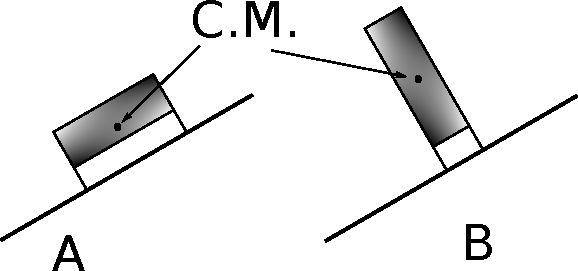
\includegraphics[width=0.45\textwidth,keepaspectratio]{tombo.pdf}
    \caption{Estudo do tombo de um corpo rígido.}
    \label{fig:tombo}
  \end{figure}
\end{ex}

\begin{ex}
  Considere um corpo rígido em um plano inclinado de superfície
  rugosa, como ilustrado na figura~\ref{fig:tombo}B. Dê argumentos que
  indiquem que o corpo não pode estar em equilíbrio (vai tombar).

  \noindent\textit{Dica:} Proceda da mesma forma que no exercício
  anterior. Mostre que o torque externo total pode ser escrito como
  $\vec\tau_{\mathrm{ext}}=\vec\tau_P+\vec\tau_N$, onde $\vec\tau_P$ e
  $\vec\tau_N$ têm a mesma direção.
\end{ex}

Suponhamos que queremos calcular o torque de uma força $\vec F$
aplicada sobre um ponto de um corpo rígido que se encontra na posição
$\vec r$ em relação a um ponto arbitrário $O$. Por definição esse
torque estará dado por $\vec\tau=\vec r\times\vec F$. Porém, às vezes
o módulo de $\vec r$ ou sua direção podem ser difíceis de se
conhecer. Para dar conta desse problema, observamos que se $\vec r'$ é
um vetor qualquer paralelo a $\vec F$, então $\vec r'\times\vec F=0$
e, por conseguinte, $\vec\tau=(\vec r+\vec r')\times \vec F$. Dessa
maneira, escolhendo o vetor $\vec r'$ de forma conveniente podemos
calcular $\vec\tau$ de forma mais simples. Em particular, se
$\vec r+\vec r'$ é um vetor perpendicular a $\vec F$, então
$\tau=|\vec r+\vec r'|F$.

\begin{ex}
  Uma barra homogênea de $12\,\mathrm{kg}$ está em equilíbrio
  estático. Um extremo dela está apoiada em uma parede rugosa e o
  outro está amarrado a uma corda como ilustrado na
  figura~\ref{fig:barra_equilibrio}. (i) Encontre o valor da tensão na
  corda. (ii) Encontre o valor da força de atrito sobre a barra devido
  à parede.
  \begin{figure}[ht]
    \centering
    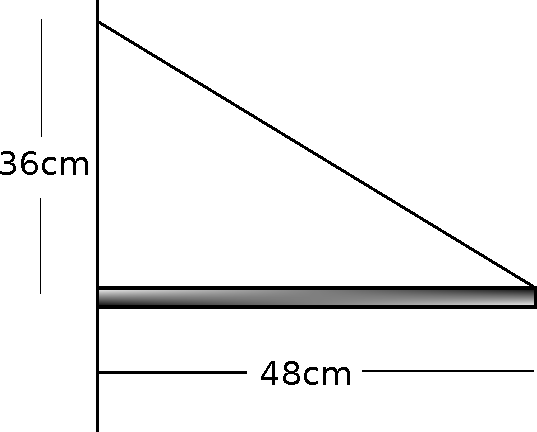
\includegraphics[width=0.45\textwidth,keepaspectratio]{barra_equilibrio.pdf}
    \caption{Barra homogênea em equilíbrio estático.}
    \label{fig:barra_equilibrio}
  \end{figure}
\end{ex}

\begin{ex}
  Uma escada homogênea de $8\,\mathrm{m}$ de comprimento e
  $5\,\mathrm{kg}$ de massa é apoiada em uma parede vertical lisa
  fazendo um ângulo de $60^\circ$ com o chão. Se uma pessoa de
  $70\,\mathrm{kg}$ está sobre a escada e ela se encontra em
  equilíbrio estático, determine o valor da força de atrito sobre a
  base da escada quando a pessoa andou na escada (i) $4\,\mathrm{m}$ e
  (ii) $6\,\mathrm{m}$.

  \noindent\textit{Dica:} Usando a primeira condição de~(\ref{eq:13}), obtenha
  que o valor da força normal sobre a base da escada é
  $735\,\mathrm{N}$. Use a segunda condição de~(\ref{eq:13}) para
  encontrar o valor da força de atrito, tomando como ponto de
  referência para o cálculo de torques o ponto de apoio da escada na
  parede.
\end{ex}

\begin{ex}
  Uma roda homogênea de massa $M$ e raio $R$ se encontra atascada
  devido a um desnível do chão. Qual deve ser o valor mínimo de uma
  força $\vec F$ horizontal aplicada no centro de massa da roda para
  que a ela comece a se mover? Esse valor mínimo é menor se a força é
  aplicada no ponto mais alto da roda?

  \noindent\textit{Dica:} Se a bola está prestes a se mover, a força
  normal devido ao chão é nula. Use a condição de equilíbrio
  $\vec\tau_{\mathrm{ext}}=0$ considerando o ponto mais alto do
  desnível como ponto de referência para o cálculo de torques.
  \begin{figure}[ht]
    \centering
    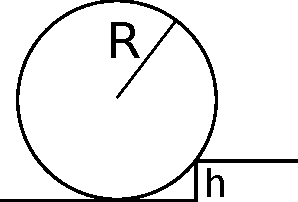
\includegraphics[width=0.45\textwidth,keepaspectratio]{roda_obstaculo.pdf}
    \caption{Roda atascada devido a um desnível do chão.}
    \label{fig:roda_obstaculo}
  \end{figure}
\end{ex}

\begin{ex}
  Quando temos um bloco homogêneo na borda de uma mesa e queremos que
  ele esteja em equilíbrio estático, o centro de massa do bloco deve
  se encontrar dentro da mesa. Considere agora dois blocos homogêneos
  de comprimento $l$. (i) Determine as condições para que ao se
  colocar um bloco sobre o outro na borda de mesa eles estejam em
  equilíbrio estático. (ii) Determine a distância máxima entre o
  extremo da mesa ao extremo do bloco superior.

  \noindent\textit{Dica:} Se $x_1$ e $x_2$ são as posições horizontais
  dos centros de massa dos blocos em relação ao bordo da mesa
  (origem), deve-se ter $x_1\le 0$, $x_2\le l+x_1$ e $x_1+x_2\le
  0$. Para maximizar a distância entre o extremo da mesa e o extremo
  do bloco $2$, nas condições anteriores devemos considerar
  $x_2=l+x_1$ e $x_1+x_2=0$.
\end{ex}

\begin{ex}
  No espíritu do exercício anterior, considere agora três blocos
  homogêneos de comprimento $l$ e determine a distância máxima entre o
  extremo da mesa ao extremo do bloco superior. Generalizando seu
  resultado, infira que ao empilhar $n$ blocos, a distância máxima
  entre o extremo da mesa e o extremo do bloco superior é dada por
  $$d=\frac{l}{2}\dpar{1+\frac{1}{2}+\frac{1}{3}+\cdots+\frac{1}{n}}\,.$$
  Mostre que usando $4$ blocos vamos ter $d>l$.

  \noindent\textit{Dica:} Primeiramente considere os dois blocos de
  cima como um bloco só e encontre as posições dos centros de massa
  desse bloco grande e do bloco de baixo. Logo, use o resultado do
  exercício anterior para colocar os dois blocos de cima de tal forma
  que $d$ tenha o maior valor possível.
\end{ex}
\end{document}